\chapter{Signal region and blinding}

Unlike the 2015 version of this analysis, which used a two-step signal region (SR) and optimization process, the current analysis uses one step, where a near-optimal SR is defined using all of the desired variables. This simplification allows for the use of the same SR for all signal models, including the same variable validation and background model. The tradeoff is a small loss in sensitivity for models with tighter optimal cuts, but the benefit of simplicity outweighs the cost of this loss. In principle, each benchmark signal point can be optimized individually to gain a few percent in sensitivity, but this is left to a future study.

Two strategies are employed to define the signal region: cut-and-count based and multivariate analysis (MVA) based. Several key discriminating variables are studied as inputs to both SR definitions: the missing transverse momentum, $\MET$, the four-lepton invariant mass, $m_{4l}$, the transverse mass of the Higgs and MET, $m_T(4l+\MET) \equiv m_T$, the difference in the transverse angle $\phi$ between the Higgs and MET, $|\Delta\phi(4l, \MET)| \equiv |\Delta\phi|$, as well as the lepton and jet multiplicities.

\subsection{Cut-and-count based signal region} \label{cutandcountopt}

The cut-and-count strategy is the simpler choice, and is used as a baseline to measure the performance of the MVA. First, the following selection is applied to isolate events with a Higgs from events with additional prompt particles (e.g. VBF Higgs production):

\begin{itemize}
\item Tight lepton multiplicity = 4
\item b jet multiplicity $\leq$ 1
\item VBF jet multiplicity $\leq$ 1
\end{itemize}

Next, the event selection is optimized by scanning over a range of cuts for the remaining variables and selecting the set of cuts that maximizes the sensitivity, measured directly by the cross section upper limit. The two variables with the greatest discriminating power between signal and background are $m_{4l}$ and $\MET$, so we maximize the sensitivity over these two variables. The best sensativity occurs where the upper limit is minimum, around:

\begin{itemize}
\item $|m_{4l} - m_H| < 10$ $\GeV$
\item $\MET > 60$ $\GeV$
\end{itemize}

These cuts define the SR, which is applied to all of the signals, losing less than 10\% sensitivity for the models with a tighter optimal cut on $\MET$. Since the signal used to defined the SR has the softest $\MET$ spectrum of all the signals, this SR corresponds to the most modest or most loose choice, meaning no signal will be cut on too hard, while most of the background is still removed. 

%\begin{figure}[tbh]
%\centering
%\includegraphics[width=3in]{figures/}
%\caption{PLACEHOLDER The optimized cut-and-count based selection for ZpBaryonic, defining the signal region for all models.}
%\label{fig:2dscan}
%\end{figure}

In addition to blinding observations of data distributions in the SR until the selection is frozen, it should be noted that there is no additional blinding on the MET distribution above a certain threshold, as was the case previously in similar searches. This is due primarily to the need to understand events that contribute large amounts of fake MET. This is covered thoroughly, including the procedure for removing these events from data, in the next section. In order to validate the modelling in these SRs, they are split into control regions (CR) based on the MET being above or below 60 $\GeV$, referred to as the high and low MET regions. 


\subsection{MVA based signal region} \label{mvaopt}

This search channel has the advantage of having backgrounds that are easily reduced by applying cuts on the discriminating variables. It was observed in the study of the 2015 data and MC samples that applying additional cuts did not improve the sensitivity since the background levels were already sufficiently low. Applying cuts on additional variables reduced the signal efficiency, which in turn reduced the sensitivity. This is also observed with 2016 MC samples, where applying the $|\Delta\phi(llll, \MET|$ does not improve the sensitivity. These observations motivate the use of MVA techniques, which can take all of the desired variables as input, but do not reduce the signal efficiency. Although it is simpler to cut on these discriminating variables as described above, there is potential for significant improvement in the sensitivity with an MVA approach.

The SR event selection is optimized for the MVA based case by training a boosted decision tree (BDT) with the ROOT TMVA package with the input variables: $m_{4l}$ and $\MET$. Including additional input features does not significantly improve the performance of the MVA. The training is done over the weighted set of backgrounds and an admixture of signal models to reduce bias toward a single signal model. The BDT response is shown in Figure~\ref{fig:bdt}, with the signal peaked toward 1 and the background peaked toward -1. 

\begin{figure}[tbh]
\centering
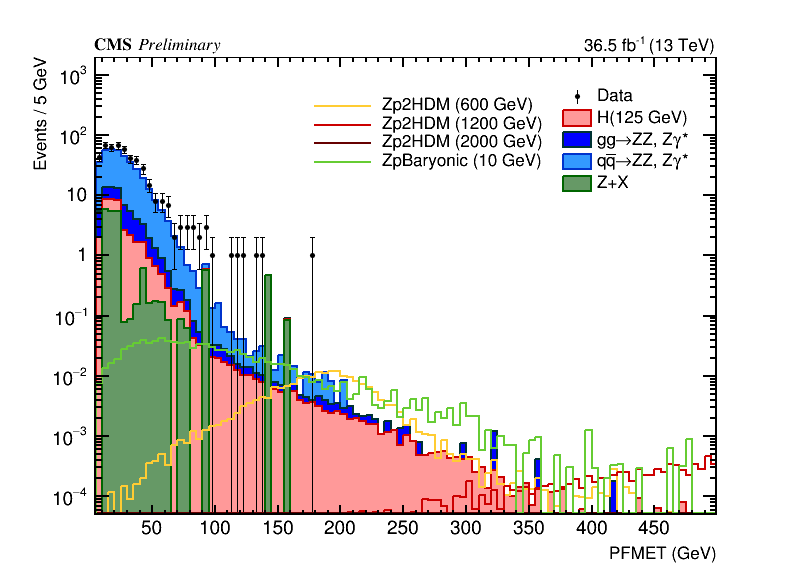
\includegraphics[width=5in]{figures/hist_hPFMET_8.png}
\caption{PLACEHOLDER BDT response.}
\label{fig:bdt}
\end{figure}


\section{Yields and distributions}

\begin{table*}[htbH]
\begin{center}
\begin{tabular}{ l | c | c | c | c}
\hline
\hline
Channel & 4e & 4$\mu$ & 2e2$\mu$ & 4$l$ \\
\hline
$q\bar{q} \rightarrow ZZ$ & 0.029 & 328 & 1.58e+03 & 1.91e+03 \\
$gg \rightarrow ZZ$ & 24.7 & 33.7 & 123 & 182 \\
$Z+X$ & 14.5 & 20.9 & 31 & 66.5 \\
$ZH$ & 0.672 & 0.905 & 1.51 & 3.09 \\
Other Higgs & 7.24 & 11 & 31.6 & 49.8 \\
\hline
Total background & 47.2 & 395 & 1.77e+03 & 2.21e+03 \\
\hline
Signal ($m_\chi=600$ GeV) & 0.143 & 0.203 & 0.349 & 0.695 \\
\hline
Total expected & 47.3 & 395 & 1.77e+03 & 2.21e+03 \\
\hline
Observed & 103 & 177 & 0 & 280 \\
\hline
\hline
\end{tabular}
\caption{PLACEHOLDER Event yields after SM selection, with $m_{4l}>70$ GeV.}\label{tab:yields}
\end{center}
\end{table*}

\begin{table*}[htbH]    
\begin{center}    
\begin{tabular}{ l | c | c | c | c | c | c | c | c }     
\hline    
\hline    
Sample & $q\bar{q} \rightarrow ZZ$ & $gg \rightarrow ZZ$ & $Z+X$ & $ZH$ & Other H & Total & Signal & Observed \\ 
\hline 
Initial & 1.19e+04 & 934 & 3.17e+08 & 17.9 & 387 & 3.17e+08 & 3.62 & 4.16e+07 \\ 
\hline 
HLT & 1.19e+04 & 934 & 3.17e+08 & 17.9 & 387 & 3.17e+08 & 3.62 & 4.16e+07 \\ 
\hline 
$Z_1$ lepton cuts & 10.3 & 130 & 3.08e+03 & 2 & 44.4 & 3.26e+03 & 0.429 & 2.3e+04 \\ 
\hline 
$m_{Z_1}$ & 7.19 & 110 & 1.87e+03 & 1.77 & 42 & 2.03e+03 & 0.404 & 1.61e+04 \\ 
\hline 
At least one $Z_2$ & 0.0327 & 53.6 & 14.5 & 0.672 & 14.3 & 83.1 & 0.143 & 103 \\ 
\hline 
$m_{Z_2}$ & 0.0327 & 53.6 & 14.5 & 0.672 & 14.3 & 83.1 & 0.143 & 103 \\ 
\hline 
$m_{ll}>4$ for OS-SF & 0.029 & 24.7 & 14.5 & 0.672 & 7.24 & 47.2 & 0.143 & 103 \\ 
\hline 
$m_{llll} > 70$ GeV & 0.029 & 24.7 & 14.5 & 0.672 & 7.24 & 47.2 & 0.143 & 103 \\ 
\hline 
\hline    
\end{tabular}    
\caption{PLACEHOLDER Cut flow for $4e$ channel. Example signal is Z'2HDM with $m_{Z'}=600$ GeV.}\label{tab:yields}    
\end{center}    
\end{table*} 

\begin{table*}[htbH]    
\begin{center}    
\begin{tabular}{ l | c | c | c | c | c | c | c | c }     
\hline    
\hline    
Sample & $q\bar{q} \rightarrow ZZ$ & $gg \rightarrow ZZ$ & $Z+X$ & $ZH$ & Other H & Total & Signal & Observed \\ 
\hline 
Initial & 1.19e+04 & 878 & 3.17e+08 & 17.9 & 387 & 3.17e+08 & 3.66 & 4.39e+07 \\ 
\hline 
HLT & 1.19e+04 & 878 & 3.17e+08 & 17.9 & 387 & 3.17e+08 & 3.66 & 4.39e+07 \\ 
\hline 
$Z_1$ lepton cuts & 2.03e+03 & 144 & 5.66e+04 & 2.37 & 57.5 & 5.89e+04 & 0.517 & 3.75e+04 \\ 
\hline 
$m_{Z_1}$ & 1.67e+03 & 128 & 4.31e+04 & 2.16 & 54.4 & 4.5e+04 & 0.486 & 1.74e+04 \\ 
\hline 
At least one $Z_2$ & 399 & 76.4 & 23 & 0.971 & 23.8 & 523 & 0.217 & 178 \\ 
\hline 
$m_{Z_2}$ & 399 & 76.4 & 23 & 0.971 & 23.8 & 523 & 0.217 & 178 \\ 
\hline 
$m_{ll}>4$ for OS-SF & 329 & 33.7 & 20.9 & 0.905 & 11 & 395 & 0.203 & 178 \\ 
\hline 
$m_{llll} > 70$ GeV & 328 & 33.7 & 20.9 & 0.905 & 11 & 395 & 0.203 & 177 \\ 
\hline 
\hline    
\end{tabular}    
\caption{PLACEHOLDER Cut flow for $4\mu$ channel. Example signal is Z'2HDM with $m_{Z'}=600$ GeV.}\label{tab:yields}    
\end{center}    
\end{table*} 

\begin{table*}[htbH]    
\begin{center}    
\begin{tabular}{ l | c | c | c | c | c | c | c | c }     
\hline    
\hline    
Sample & $q\bar{q} \rightarrow ZZ$ & $gg \rightarrow ZZ$ & $Z+X$ & $ZH$ & Other H & Total & Signal & Observed \\ 
\hline 
Initial & 3.7e+04 & 934 & 3.28e+06 & 17.9 & 387 & 3.32e+06 & 3.62 & 0 \\ 
\hline 
HLT & 3.7e+04 & 934 & 3.28e+06 & 17.9 & 387 & 3.32e+06 & 3.62 & 0 \\ 
\hline 
$Z_1$ lepton cuts & 8.73e+03 & 422 & 4.71e+03 & 5.83 & 136 & 1.4e+04 & 1.33 & 0 \\ 
\hline 
$m_{Z_1}$ & 6.96e+03 & 369 & 2.98e+03 & 5.3 & 127 & 1.04e+04 & 1.23 & 0 \\ 
\hline 
At least one $Z_2$ & 1.58e+03 & 123 & 31 & 1.51 & 31.6 & 1.77e+03 & 0.349 & 0 \\ 
\hline 
$m_{Z_2}$ & 1.58e+03 & 123 & 31 & 1.51 & 31.6 & 1.77e+03 & 0.349 & 0 \\ 
\hline 
$m_{ll}>4$ for OS-SF & 1.58e+03 & 123 & 31 & 1.51 & 31.6 & 1.77e+03 & 0.349 & 0 \\ 
\hline 
$m_{llll} > 70$ GeV & 1.58e+03 & 123 & 31 & 1.51 & 31.6 & 1.77e+03 & 0.349 & 0 \\ 
\hline 
\hline    
\end{tabular}    
\caption{PLACEHOLDER Cut flow for $2e2\mu$ channel. Example signal is Z'2HDM with $m_{Z'}=600$ GeV.}\label{tab:yields}    
\end{center}    
\end{table*} 

